\documentclass[12pt]{book}
\usepackage{graphicx}
\usepackage{amssymb}
\usepackage{multicol}
\usepackage{ifthen}
\usepackage{color}
\usepackage{setspace}
\usepackage{amsthm, amsmath}
\usepackage{pdfpages}
\usepackage{tikz}
\usepackage{url}

\usepackage{geometry}
\geometry{papersize={8.5in,11in}, hmargin={1.25in, 1.25in}, bindingoffset=0.25in, height=8.5in, top=1in, headheight=15pt, twoside, ignoreheadfoot}

% No section numbers:
\setcounter{secnumdepth}{0}

\doublespacing

\newtheorem{theorem}{Theorem}

\theoremstyle{definition}
\newtheorem{definition}{Definition}
\newtheorem{example}{Example}

\def\Z{\mathbb{Z}}

\usepackage[utf8]{inputenc}
\usepackage[T1]{fontenc}
\usepackage{newpxtext}
\usepackage[vvarbb,cmintegrals,cmbraces,bigdelims]{newpxmath}
\usepackage[scr=rsfso]{mathalfa}% \mathscr is fancier than \mathcal
% \linespread{1.04}         % adds more leading (space between lines)
% quantifiers look strange, so change those back to normal:
	\DeclareSymbolFont{mysymbols}{OMS}{cmsy}{b}{n} %note we make the figures bold to better match newpx.  Replace the ``b'' with an ``m'' to undo this.
	%\SetSymbolFont{mysymbols}  {bold}{OMS}{cmsy}{b}{n}
	%\DeclareSymbolFont{myoperators}   {OT1}{cmr} {m}{n}
	%\SetSymbolFont{myoperators}{bold}{OT1}{cmr} {bx}{n}
	\DeclareMathSymbol{\forall}{\mathord}{mysymbols}{"38}
	\DeclareMathSymbol{\exists}{\mathord}{mysymbols}{"39}
	%\DeclareMathSymbol{\pm}{\mathbin}{mysymbols}{"06}
	%\DeclareMathSymbol{+}{\mathbin}{myoperators}{"2B}
	%\DeclareMathSymbol{-}{\mathbin}{mysymbols}{"00}
	%\DeclareMathSymbol{=}{\mathrel}{myoperators}{"3D}

%%%%%%%%%%%%%%%%%%%%%%%%%%%%%%%%%%%%%%%%%%
%%%%%%%  Headers and footers %%%%%%%%%%%%%
%%%%%%%%%%%%%%%%%%%%%%%%%%%%%%%%%%%%%%%%%%
\usepackage{fancyhdr}
\pagestyle{fancy}
\renewcommand{\chaptermark}[1]{\markboth{\thesection.\ #1}{}} %Removes word "chapter" from the \leftmark.


\fancyhead{} % clear header fields
\fancyhead[LE]{{\footnotesize \textsl{\thepage}}~~ \textsc{\scriptsize \nouppercase{\leftmark}}}
\fancyhead[RO]{\textsc{\scriptsize \nouppercase{\rightmark}} ~~ {\footnotesize \textsl{\thepage}}  }
\fancyfoot{}

%%%%%%%%%%%%%%%%%%%%%%%%%%%%%%%%%%%%%%%%%%
%%%%%%%    Chapter headings  %%%%%%%%%%%%%
%%%%%%%%%%%%%%%%%%%%%%%%%%%%%%%%%%%%%%%%%%

\usepackage[bf,sc,center,outermarks]{titlesec}


%%%%% FIX FOR BUG IN TITLESEC %%%%%%%%%%%
\usepackage{etoolbox}

\makeatletter
\patchcmd{\ttlh@hang}{\parindent\z@}{\parindent\z@\leavevmode}{}{}
\patchcmd{\ttlh@hang}{\noindent}{}{}{}
\makeatother
%%%%% END FIX %%%%%%%%%%%%%%%%%%%%%%%%%%%%


% \titleformat{\chapter}[display]
% 	{\Large\filcenter}
% 	{\rule[4pt]{.3\textwidth}{2pt} \hspace{2ex} \large\textsc{\chaptertitlename} \thechapter \hspace{3ex} \rule[4pt]{0.3\textwidth}{2pt} }
% 	{1pc}
% 	{\titlerule\vspace{1ex}\huge\textsc}
% 	[\vspace{.75ex}\titlerule]
% \titlespacing*{\chapter}{0pt}{-2em}{2em}

\titleformat{\subsection}[block]
  {\normalfont\bfseries\filcenter}
  {\theparagraph}
  {}
  {\textsc}

\newcommand{\sectionbreak}{\clearpage\thispagestyle{plain}}
\titleformat{\section}[block]
  {\Large\bfseries\filcenter}
  {\theparagraph}
  {}
  {\textsc}
%%%%%%%%%  End chapter/sectio headings %%%%%%%%%%%%%%%%%


\begin{document}

\pagestyle{plain}
\pagenumbering{roman}




\thispagestyle{empty}


%~
%\tikz[remember picture, overlay] \node  at (current page.center){\includegraphics[width=\paperwidth,height=\paperheight]{images/titlebg}};


~
\vskip 1.75in

\begin{center}


\resizebox{.9\linewidth}{!}{\scshape Some Abstract Algebra}


\vskip 3em

% \tikz[scale=1]{
% \draw (0,0) rectangle (2,2);
% \draw (-0.2, -0.2) rectangle (2.2, 2.2);
% \draw (-0.4, -0.4) rectangle (2.4, 2.4);
% \draw (-0.6, -0.6) rectangle (2.6, 2.6);
% }

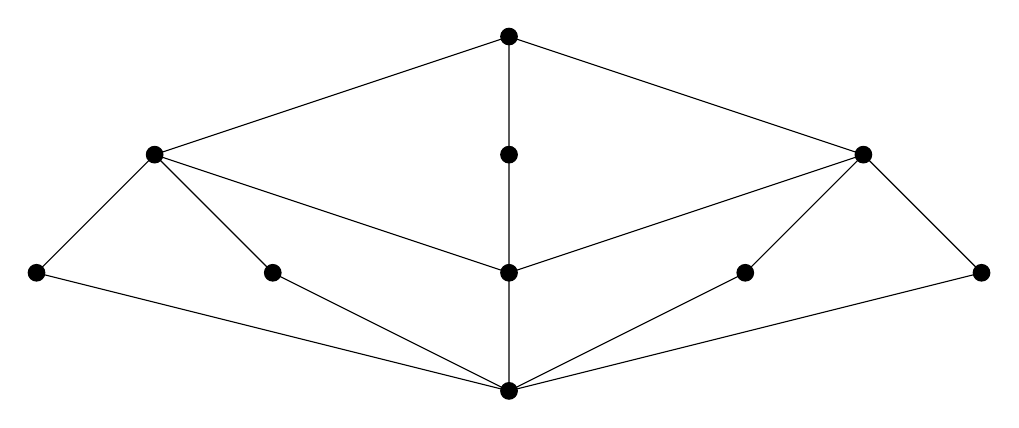
\begin{tikzpicture}[scale=1.5]
	\coordinate (h9) at (0,0);
	\coordinate (h8) at (4,1);
	\coordinate (h7) at (2,1);
	\coordinate (h6) at (0,1);
	\coordinate (h5) at (-2,1);
	\coordinate (h4) at (-4,1);
	\coordinate (h3) at (3,2);
	\coordinate (h2) at (0,2);
	\coordinate (h1) at (-3,2);
	\coordinate (h0) at (0,3);

	\draw[color=black] (h0) -- (h1) -- (h4) -- (h9) -- (h8) -- (h3) -- (h0) -- (h2) -- (h6) -- (h9) -- (h5) -- (h1) -- (h6) -- (h3) -- (h7) -- (h9);
	\foreach \i in {0,...,9}{
	\draw[fill=black, color=black] (h\i) circle (2pt);
	}
\end{tikzpicture}

\vskip 2em

\resizebox{.75\linewidth}{!}{\scshape A Primer and Interactive Workbook}



\vskip 1.5in

\resizebox{.75\linewidth}{!}{\scshape Richard Grassl \quad - \quad Tabitha Mingus}

\vskip .5in

% \resizebox{.2\linewidth}{!}{\scshape 2018}

\end{center}


%\includepdf[pages=-,pagecommand={\thispagestyle{empty}}]{frontmatter/cover2}
%
%

\clearpage






%\addtocontents{toc}{\protect\thispagestyle{plain}}

\thispagestyle{empty}
\vskip 1em

\noindent Richard Grassl \\[-1.5ex] Emeritus Professor of Mathematical Sciences \\[-1.5ex] University of Northern Colorado \\[-1.5ex] Greeley, Co 80639 \\[-1.5ex] \url{richard.grassl@unco.edu}

\vskip 1em

\noindent Tabitha Mingus \\[-1.5ex] Associate Professor of Mathematics \\[-1.5ex] Western Michigan University \\[-1.5ex] Kalamazoo, MI 49008


\vfill
\vfill
\noindent\textcopyright ~ 2018 by Richard Grassl

\vskip 3em

\noindent
\includegraphics[scale=.5]{frontmatter/by-sa}\\
This work is licensed under the Creative Commons Attribution-ShareAlike 4.0 International License. To view a copy of this license, visit\\ \url{http://creativecommons.org/licenses/by-sa/4.0/}.

\vfill

\noindent Summer 2018 Edition
\vskip 1em
% \noindent ISBN-10: 1534970746\\
% \noindent ISBN-13: 978-1534970748

\vfill

\noindent A current electronic version can be found for free at\\ \url{http://www.openmathbooks.org/someabstract/}
\vskip 2em

% \noindent Cover image: \emph{Tiling with Fibonacci and Pascal}.
\noindent Prepared for publication by Oscar Levin for Open Math Books
\vskip 2em

\clearpage


\section*{Preface}

This book consists of two parts: one, a primer designed to provide an adequate introduction to the essentials of abstract algebra and to some related number theory, and two, a workbook designed to enable the reader to interactively engage with colleagues in exploring the fascinating world of abstract algebra.

We have taken a problem solving approach -- the primer alone contains over 130 problems. So be prepared for minimal text material to read, combined with worksheets that extend and enhance text topics. These worksheets are designed to encourage discovery of interesting relationships between algebraic structures, geometry, mappings, and proofs.

Very little, if any, background in abstract algebra is needed for a course based on this Primer and the workbook. This material has been used successfully for over a decade with in-service secondary teachers seeking licensure or an MA degree in teaching mathematics.

In this book we embrace the oft-quoted maxim - ``You learn mathematics by doing mathematics.'' Such an effort leads to better understanding and deeper learning.

Finally, a valuable by-product: A significant number of teachers who have studied this material have incorporated a variety of the worksheets into their secondary curriculum as they encounter topics like closure, binary operations and their properties, modular arithmetic, and the structure of the integers (yes, GCD and LCM show up), and the rational and real numbers.

% This book is rebound under an open source license and is available in electronic format for free at \url{http://www.openmathbooks.org/someabstract/}.

\begin{flushright}
  Richard Grassl\\
  April 2019
\end{flushright}


\cleardoublepage


 \thispagestyle{empty}
\centerline{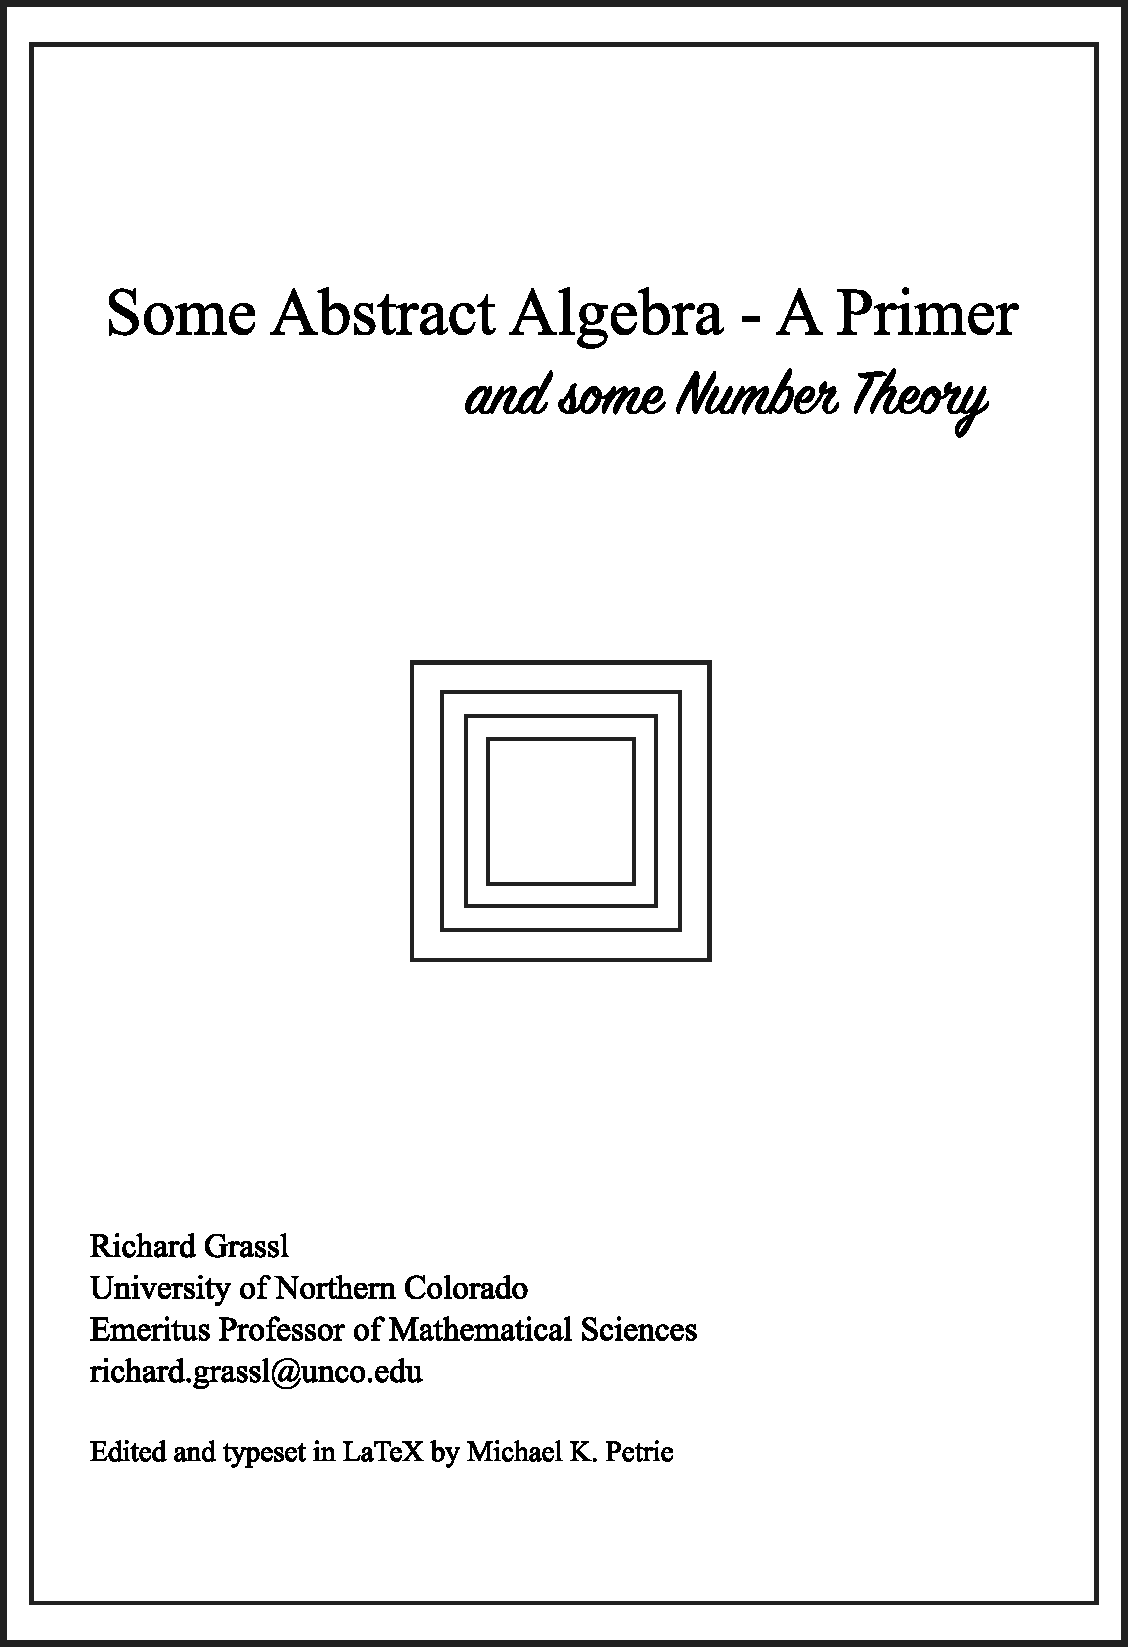
\includegraphics[width=6in]{Coverpage.pdf}}

% \rule{0in}{1in}\\
% \rule{.75in}{0in}\begin{minipage}{5in}

% \end{minipage}
\clearpage
\setcounter{tocdepth}{1}
% \rule{0in}{2in}\\

% \begin{minipage}{4in}
\tableofcontents
% \end{minipage}
\cleardoublepage
\pagenumbering{arabic}

\pagestyle{fancy}

\section*{Introduction}
An abstract algebra consists of a set of objects (integers, real numbers, permutations, polynomials, matrices, $\dots$), various binary operations, along with some properties (closure, inverses, commutativity,$\dots$). Examples of abstract algebras include groups, rings, integral domains, and fields. Operations include rotations of regular geometrical figures, ordinary and modular addition and multiplication, addition and multiplication of matrices and of polynomials, composition of permutation cycles, direct products and others.

In one sense the core ideas of algebra are abstracted out and viewed from a much larger lens. For example, the problem of finding analogues of the quadratic formula, around the mid 1500’s, led to the study of the symmetric groups which shed light on the nonsolvability of the general quintic.

Applications are plentiful. Among the many fields of study making significant use of algebraic structures we include cryptography, genetics, mineralogy, the study of molecular structures in chemistry, elementary particle theory in physics, Latin squares in statistical experiments, and finally, architecture and art.

Important contributors over the past several centuries include Joseph Lagrange, Niels Abel, Arthur Cayley, Emmy Noether, Gauss, Galois, Sylow among many others.
\cleardoublepage

\section{Closure}

\quad We say that a binary operation $\square$ on a set $S$ is CLOSED if whenever $a$ and $b$ are any two elements in $S$ then $a\,\square\, b$ is also in $S$.  For example, the operation $+$ is closed on the set $S=Z=\{0,\pm1,\pm2,\dots\}$ since $a+b$ is in $Z$.  But subtraction is not closed on the set $N=\{0,1,2,3,\dots\}$ since $1-3=-2$ is not in $N$.

The following gives the two part procedure for determining if a particular set $S$ is closed under a particular binary operation $\square$:
\begin{enumerate}
\item Choose two arbitrary elements for $S$; label them $a,\,b$.
\item Show that $a\,\square\, b$ is a number of $S$.
\end{enumerate}
\underline{Example.} The set $E=\{0,2,4,6,\dots\}$ is closed under addition.  Let $a=2m$ and $b=2n$ be arbitary elements of $E$.  Then since $2m+2n=2(m+n)$ is an even integer the sum of $2m$ and $2n$ is in $E$.  $E$ is also closed under multiplication since $(2m)(2n)=4mn=2(2mn)$ is even.\\[.1 in]
\underline{PROBLEMS.}

In each of the following if the set is closed under the operation give reasons (actually a proof); if not, provide a counterexample.\\[.1in]
\begin{enumerate}
\item Is $A=\{0,1,4,9,16,\dots\}$ closed\\
a. under addition?\qquad b. under subtraction? \qquad c. under multiplication?
\item Is $B=\{0,\pm5,\pm10,\pm15,\dots\}$ closed\\
a. under addition?\qquad b. under multiplication?
\item Is $C=\{0,2,4,6\}$, a finite set, closed under addition?
\item Is $D=\{1,3,5,7,\dots\}$ closed\\
a. under addition?\qquad b. under multiplication?
\item Is $E=\{1,4,7,10,13,\dots\}$, the positive integers having remainder 1 upon division by 3 closed\\
a. under addition?\qquad b. under multiplication?
\item Repeat \#5 with $F=\{2,5,8,11,14,\dots\}$.
\item The set $G=\{0,\pm4,\pm8,\pm12,\dots\}$ is closed under subtraction.  Give another set $H$ that is closed under subtraction.  Show that $G\cap H$ is also closed under subtraction.
\item Is the set of all rational numbers of the form $2^n$, where $n$ is in $Z$, closed under multiplication?
\item Is the set of all positive rational numbers closed under addition?  Under multiplication?
\item Let $I=\{2^m\cdot3^n:m,n \text{ are in } Z\}$.  Is $I$ closed under multiplication?\\
Hint:  Is 3/8 in $I$?  Is 1/9 in $I$?
\item Are the irrationals closed under multiplication?
\item Prove that if $S$ and $T$ are sets of integers closed under subtraction so is the intersection $S\cap T$.  Is the union of $S$ and $T$ also closed under subtraction?
\item Why does 0 always have to be a member of any set that is closed under subtraction?
\item Let $R$ denote a $120^\circ$ rotation of an equilateral triangle.  Is the set $\{I,R,R^2\}$ closed under ``rotation''?  Here, $I$ means do nothing and $R^2$ means a $240^\circ$ rotation.
\end{enumerate}
\subsection{Units Multiplication}

Under units multiplication the product of any two positive integers, denoted by $a\,\square\, b$, is the units digit of the product under ordinary multiplication.  So $5\,\square\,9=5,\, 7\,\square\,8=6$.
\begin{enumerate}
\item[15.] Is the set $\{0,2,4,6,8\}$ closed under units multiplication?
\item[16.]Is the set $\{1,3,7,9\}$ closed under units multiplication?
\item[17.]Is $\{1,4,6\}$ closed under units multiplication?  How about the set $\{2,4,8\}$?  How about $\{1,5,9\}$?
\item[18.]What would you have to add to the set $\{1,3,5\}$ to make it closed under units multiplication?
\end{enumerate}


\section{Binary Operations}
\quad The concepts of being commutative and associative are usually introduced to students as they study the four basic arithmetic operations of addition, subtraction, multiplication and division of integers.  These four operations denoted by $+,\,-\,\times,\, \div$ are examples of binary operations.\\[.1in]

Let $S$ be any set.  A \underline{binary operation} on $S$ is  a function $f:S\times S\mapsto S$.  Sometimes a binary operation is depicted using the \underline{infix} notation $(m,n)\rightarrow m\,\square\, n$, rather than the \underline{prefix} notation$f(m,n)$.  The following are examples of binary operations on $N=\{0,1,2,3,\dots\}$.\\
$$\begin{array}{|c|c|}
\hline
\underline{\text{OPERATION}}&\underline{\text{INFIX NOTATION}}\\
\hline
f(m,n)=m+n & m\,\square\, n=m+n\\
\hline
f(m,n)=mn & m\,\square\, n=mn\\
\hline
f(m,n)=\text{GCD}(m,n) & m\,\square\, n=\text{GCD}(m,n)\\
\hline
f(m,n)=5^m\cdot n & m\,\square\, n=5^m\cdot n\\
\hline
\end{array}$$
Additional binary operations that will be of importance include
\begin{equation*}\begin{split}
f(x,y)&= x\div y \text{ on }S=\text{Reals}\\
f(m,n)& = m-n \text{ on } S=Z=\{0,\pm1,\pm2,\dots\}\\
f(m,n)&=m+n-mn \text{ on }S=Z\\
f(m,n)&=m+n-1 \text{ on }S=Z\\
f(A,B)&=A\cup B \text{ on } P(S) \text{ for }S=\{\text{a,b,c}\}\\
f(A,B)&=A\cap B \text{ on } P(S) \text{ for }S=\{\text{a,b,c}\}
\end{split}\end{equation*}
Here, $\cup$ denotes union and $\cap$ denotes intersection.  Also, $P(S)$, the power set for $S$, is the set of all subsets of $S$.  As an example, if $S$=\{a,b\},then $P(S)$ = \{ $\emptyset$, \{a\}, \{b\}, \{a,b\} \}.\\[.1in]

\subsection{Properties of Binary Operations}

Binary operations on a set $X$ may or may not satisfy the following properties:\\
\underline{Commutativity:} $x\,\square\, y =y\,\square\, x$ for all $x,y$ in $X$.\\
\underline{Associativity:} $x\,\square\,(y\,\square\, z)=(x\,\square\, y)\,\square\, z$ for all $x,y,z$ in $X$.\\
\underline{Identity:} An element $e\in X$ such that $x\,\square\, e=e\,\square\, x = x$ for $x$ in $X$ is called an identity for the binary operation $\square$.\\
\underline{Inverses:} If $e$ is an identity under $\square$, an inverse of an element $a$ in $X$ is an element $b$ in $X$ such that $a\,\square\, b=e=b\,\square\, a$.\\
\underline{Example 1.}  The operation $+$ on $Z$ is associative since $a+(b+c)=(a+b)+c$ for all $a,b,c$ in $Z$.  Since $a+b=b+a$, + is commutative.  The element 0 serves as an identity $e$ since $0+a=a+0=a$.  Each element $a\in Z$ has an inverse, namely $-a$.\\[.1in]

One important characterization or consequence of the notation $f:A\times A\mapsto A$ is that the result $f(m,n)$, or $m\,\square\, n$, must be an element in $A$; i.e., $A$ must be \underline {closed} under the binary operation $\square$.  So divisibility, denoted $\div$, is not a binary operation on $N=\{0,1,2,\dots\}$ since $m\div n = \frac m n$ is not necessarily an integer.  But $\div$ is a binary operation on the set $R^+$ of positive real numbers.  Notice that since $2\div3\neq3\div2$, $\div$ is not commutative.\\[.5in]

Consider the binary operation $m\,\square\, n=3^m\cdot n$ on $N=\{0,1,2,\dots\}$; show that $\square$ is \underline{not} associative.  The following single example accomplishes this:
$$1\,\square\,(0\,\square\, 1) = 1\,\square\, 1 = 3\text{ but }(1\,\square\, 0)\,\square\, 1 = 0\,\square\, 1 = 1$$
Does $\square$ have an identity?  it might be natural to try 0 or 1.  Since $0\,\square\, n = n$ but $n\,\square\, 0=0$, 0 is not an identity.  Since $1\,\square\, n = 3n$, 1 is not an identity.  No other element in $n$ works either;  without an identity, there are no inverses.\\[.5in]
\underline{Example 2.}  Union, $\cup\,$, is a binary operation on $P(S)$ where $S$=\{a,b,c\}.  Since $A\cup(B\cup C)=(a\cup B)\cup C$, $\cup$ is associative.   Since $\emptyset \cup A=A=A\cup\emptyset$ for all $A\in P(S)$, the empty set $\emptyset$ serves as an identity.\\[.25in]
When the set $A$ is finite, a binary operation $\square$ can be given by a matrix table where the element $x\,\square\, y$ is found at the intersection of row $x$ and column $y$.

\underline{Example 3.} Let $A=\{1,3,7,9\}$ and let $x\,\square\, y$ be the digit in the units position upon ordinary multiplication of $x$ and $y$.  This is sometimes written as $x\,\square\, y \equiv xy(\text{mod }10)$.  The matrix table is
$$\begin{array}{c|cccc}
\,\square\, & 1 & 3 & 7 & 9\\
\hline
1 & 1 & 3 & 7& 9\\
3 & 3 & 9 & 1& 7\\
7 & 7 & 1 & 9 & 3\\
9 & 9 & 7 & 3 & 1
\end{array}$$
This binary operation $\,\square\,:A\times A\mapsto A$ is associative (you need to check $4\cdot4\cdot4=64$ cases), is commutative (from the symmetry of the table), has identity 1, and each element has an inverse as shown in the following table:
$$\begin{array}{c|cccc}
x & 1 & 3 & 7 & 9\\
\hline
\text{inverse of }x & 1 & 7 & 3 & 9
\end{array}$$%
%
\underline{Example 4.} The binary operation $\circ$ on $A$=\{e, a, b\} given by the table below is associative, commutative and has e as an identity.  In the exercises you are asked to find inverses.\\
\begin{minipage}{2in}
$$\begin{array}{c|ccc}
\,\circ\, & \text{e} &\text{a} & \text{b}\\
\hline
\text{e} & \text{e} & \text{a} & \text{b}\\
\text{a} & \text{a} & \text{b} & \text{e}\\
\text{b} & \text{b} & \text{e} & \text{a}
\end{array}$$
\end{minipage}
\begin{minipage}{3.5in}
$$\begin{array}{c|cccc}
\,\square\, & 1 & 2 & 5& 10\\
\hline
1 & 1 & 1 & 1 &1\\
2 & 1 & 2 & 1 & 2\\
5 & 1 & 1 & 5 & 5\\
10 & 1 & 2 & 5 & 10
\end{array}$$
\end{minipage}\\[.1in]
\underline{Example 5.}  Let $A=\{1,2,5,10\}$ and $m\,\square\, n = \text{GCD}(m,n)$, the greatest common divisor of $m$ and $n$.  The matrix table for $\square$ is given.  With some effort, you can show that $\square$ is associative.The table's symmetry verifies that the operation $\square$ is commutative.  In the exercises, you are asked to determine an identity and to see if there are inverses.\\[.1in]

\subsection{``An'' Identity versus ``The'' Identity}
Throughout this discussion of properties we have been saying ``an'' identity.  Here is some good news!  We can replace ``an'' with ``the'' whenever an identity exists.\\[.5in]
\underline{Theorem:} If the binary operation $\square$ on $X$ has an identity, then it is unique.\\
\underline{Proof:} Proceed using a proof by contradiction.  Suppose there are two different identities; call them $e$ and $f$.  Since $x\,\square\, e=x=e\,\square\, x$ for all $x$ in $X$, it must hold for $x=f$, i.e., $f\,\square\, e= f = e\,\square\, f$.  Since $x\,\square\, f=x=f\,\square\, x$ for all $x$ in $X$, it must hold for $x=e$, i.e., $e\,\square\, f=e=f\,\square\, e$.  But then $e\,\square\, f=f$ and $e\,\square\, f =e$, or $e=f$ contradicting the fact that they were different.\\[.1in]

Similarly inverses are  unique.  Let $e$ be the identity for an associative operation $\circ$ on $X$, and let $g$ and $h$ be two inverses for some $a$ in $X$.  Then $g=g\,\circ\, e=g\,\circ\,(a\,\circ\, h)=(g\,\circ\, a)\,\circ\, h=e\,\circ\, h = h$.  You should give reasons for each step.\\[.1in]

\subsection{Meet and Join}
There are two binary operations on $B$=\{0,1\} that are basic in computer design and operation.  The \underline{meet} $\bigwedge$ and \underline{join} $\bigvee$operations are given by the tables below.\\[.3in]
\begin{minipage}{3in}
$$\begin{array}{c|cc}
\bigwedge & 0 & 1\\
\hline
0 & 0 & 0\\
1& 0 & 1\\
\end{array}$$
\end{minipage}
\begin{minipage}{3.5in}
$$\begin{array}{c|cc}
\bigvee & 0 & 1\\
\hline
0 & 0 & 1\\
1& 1 & 1\\
\end{array}$$
\end{minipage}\\[.3in]
The meet operation is similar to intersection $\cap$ and join is similar to union $\cup$, and behave like the logical connectives ``and'' and ``or'' respectively.  Each of $\bigwedge$ and $\bigvee$ are commutative and associative.  Are there identities, inverses?

\subsection{Bitwise Addition Modulo 2}

Another binary operation having applications in coding theory is based on the table below.\\[.1in]
$$\begin{array}{c|cc}
\oplus & 0 & 1\\
\hline
0 & 0 & 1\\
1 & 1 & 0\\
\end{array}$$
\rule{0in}{.1in}
Here, $a\,\oplus\,b$ is 0 if $a+b$ is even and $a\,\oplus\,b=1$ if $a+b$ is odd.  Equivalently, $a\,\oplus\,b=0$ if $a=b$, and $a\,\oplus\,b=1$ if $a\neq b$.  The binary operation $\oplus$ on $B=\{0,1\}$ is called ``bitwise addition modulo 2''.  On $B^2=\{00,01,10,11\}$, the table for $\oplus$ is given. \\[.1in]
\begin{minipage}{3.5 in}
The operation is performed bitwise; $10\,\oplus\,01=11$ since $1\,\oplus\,0=1$ and $0\,\oplus 1 =1$.  You are asked to investigate properties of $\oplus$ in the exercises.
\end{minipage}
\begin{minipage}{3.5in}
$$\begin{array}{c|cccc}
\oplus& 00 & 01 & 10 & 11\\
\hline
00 & 00 & 01 & 10 & 11\\
01 & 01 & 00 & 11 & 10\\
10 & 10 & 11 & 00 & 01\\
11 & 11 & 10 & 01 & 00
\end{array}$$
\end{minipage}

\underline{PROBLEMS.}
\begin{enumerate}
\item (a) Is subtraction a commutative binary operation on $Z$?  Explain.
\begin{enumerate}
\item[(b)] Is subtraction associative on $Z$?
\item[(c)]  is multiplication commutative on $Z$?
\item[(d)]  Does multiplication have an identity on $Z$?  Are there inverses?
\end{enumerate}
\item Give an example of subsets $A$ and $B$ of $Z$ so that
\begin{enumerate}
\item subtraction is not a binary operation on $A$.
\item multiplication is not a binary operation on $B$.
\end{enumerate}
\item Let $S$=\{a,b,c\}, and $P(S)$ be the power set of $S$.
\begin{enumerate}
\item Is $\cup$ on $P(S)$ commutative  Explain.
\item Does \{a\} have an inverse?
\end{enumerate}
\item Let $S$=\{a,b,c,d\}.
\begin{enumerate}
\item Is $\cap$ on $P(S)$ commutative, associative?  Explain.
\item Does $\cap$ have an identity?
\item What is the inverse of $A$=\{b,d\} under $\cap$?
\end{enumerate}
\item Let $\circ$ be the binary operation on $N=\{0,1,2,3,\dots\}$ with $m\,\circ\,n = (5^m)(2n+1)$.
\begin{enumerate}
\item Compute $2\,\circ\, 3$ and $ 3\,\circ\,2$.  Is $\circ$ commutative?
\item Is $\circ$ associative?  Does $\circ$ have an identity?
\end{enumerate}
\item Let $\circ$ be the binary operation $m\,\circ\,n=m+n-mn$ on $Z$.  Is $\circ$ commutative, associative?  Does $\circ$ have an identity?
\item Make a table of inverses for the operation in example 4.
\item Let $A=\{1,-1,i,-i\}$ and let $\square$ denote ordinary complex multiplication.\\
(a) Make the matrix table for $\square$.\qquad (b) Is $\square$ associative, commutative?\\
(c) Does $\square$ have an identity?\\
(d) Give a table of inverses for the elements of $A$.
\item What is the identity for the binary operation in example 5?  Are there inverses?
\item Let $A=\{1,2,5,10\}$ and define a binary operation on $A$ by $m\,\square\,n = \text{LCM}(m,n)$.  Make the matrix table for $\square$ and decide whether $\square$ is commutative, has an identity, inverses.
\item Let $A=Z=\{0,\pm1, \pm2,\pm3,\dots\}$ and define a binary operation on $Z$ by $m\,\square\,n=m+n-1$.\\
(a) Is $\square$ commutative?\qquad (b) Does $\square$ have an identity?\\
(c) Are there inverses?
\item Define the operation $\square$ on $Z^+$ as follows: $m\,\square\,n = \text{GCD}(m,n)+\text{LCM}(m,n)$.  Is $\square$ associative?
\item (a) Is $m\,\square\,n=3^m\cdot n$ commutative on $N=\{0,1,2,3,\dots\}$?\\
(b) How many ordered pairs $(m,n)$ can you find so that $m\,\square\,n = 18$?
\item Which properties are satisfied by $\oplus$, bitwise addition modulo 2?
\item Show that $m\,\square\,n = n\,2^m$ is not associative on $N=\{0,1,2,\dots\}$.  Is $\square$ commutative?
\item Let $m\,\circ\,n = m+n-3$ on $Z$.  What is the identity?  What is the inverse of an element $p$?
\end{enumerate}

\section{Groups}
\quad A group is an algebraic structure that consists of two items: a set of elements $G$, and a binary operation $\circ$.  This structure satisfies FOUR axioms:\\
\underline{CLOSURE:} For any elements $a$ and $b$ in $G$, $a\,\circ\,b$ is also in $G$.\\
\underline{IDENTITY:} There is a unique element $e$ in $G$ such that for any $a\in G$ we have $a\,\circ\,e=a=e\,\circ\,a$.
\underline{INVERSES:} For every element $a$ in $G$ there is an element $a^{-1}$ in $G$ so that $a\,\circ\,a^{-1}=e=a^{-1}\,\circ\,a$\\
\underline{ASSOCIATIVITY:} For any three elements $a, b, c$ in $G$ we have $(a\,\circ\,b)\,\circ\,c=a\,\circ\,(b\,\circ\,c).$\\
A general group can be denoted as $(G,\circ)$ indicating the importance of having both a carrier set $G$ and a binary operation $\circ$.  When the operation is clear from a particular context we may write just $G$ for that group.\\[.1in]
\underline{Example 1.} $(Z,+)$ is a group under the usual addition operation.  Choose $a,b$ in $Z$.  Since $a+b$ is an integer CLOSURE holds.  The identity $e$ is 0 since $0+a=a=a+0$ for any $a\in G$.  The inverse of $a$ is $-a$ (we could write $a^{-1}=-a$) since $a+(-a)=0=(-a)+a$.  ASSOCIATIVITY holds since $(a+b)+c = a+(b+c)$.\\[.1in]
\underline{Example 2.}  In the exercises you will show that the following are groups: $(Q,+)$, $(R,+)$, $(Q^+,\times)$, $(R^+,\times)$ where $Q$=Rationals, $R$=Reals, $Q^+$=positive Rationals, $R^+$=positive Reals.\\[.1in]
\underline{Example 3.} In the exercises you will show that the following are \underline{not} groups: $(Z,-),\,(Z,\div)$.\\[.1in]

\subsection{Abelian Groups}
\rule{0in}{.5in}
Some groups have an additional fifth property called commutativity.  A binary operation $\circ$ on a set $G$ is commutative if $a\,\circ\,b = b\,\circ\,a$ for all $a,b$ in $G$.  We also say that the group $(G,\circ)$ is an abelian group, named after Niels Abel, a major contributor in the development of group theory.  He also proved the insolvability of the fifth-degree polynomial equation, one of his greatest achievements.

The examples involving $Z,\, Q$, and $R$ above are all abelian groups.

\subsection{Group Tables}
\rule{0in}{.1in}
When the set $G$ is finite (most of the above examples were infinite) the four group properties and be readily detected from an operation table. We saw earlier that the set $G=\{1,3,7,9\}$ was closed under units multiplication denoted $\otimes$.  The operation table follows.
$$\begin{array}{c|cccc}
\otimes & ~1~& ~3~ & ~7~ & ~9~\\
\hline
1 & 1 & 3 & 7 & 9\\
3 & 3 & 9 & 1 & 7\\
7 & 7 & 1 & 9 & 3\\
9 & 9 & 7 & 3 & 1
\end{array}$$
The symbol $\otimes$ means take $a$ from the left most column and ``multiply'' by $b$ from the very top row.  The 16 interior elements are just 1, 3, 7 and 9 showing \underline{closure}.  The element 1 acts like the \underline{identity}  -- look at the top interior row and the left most interior column.  \underline{Inverses} are easy to find;  just look for the 1's in the table.  Since $1\,\otimes\, 1=1,\,3\,\otimes\,7=1$ and  $9\,\otimes\,9=1$ we have the following table of inverses.
$$\begin{array}{c|cccc}
x & 1 & 3 & 7 & 9\\
\hline
x^{-1} & 1 & 7 & 3 & 9
\end{array}$$
\underline{Associativity} is inherited from multiplication in $Z$; we now know that $(G,\otimes)$ is a group.  in fact, the symmetry of the table shows that $G$ is an abelian group.\\[.1in]
\underline{Example 4.}  Here is an example of a group that involves functions and algebra.  The operation is composition of functions.  Let $f(x)=x$, $g(x)=\frac{1}{1-x}$ and $h(x)=\frac{x-1}{x}$.  $G=\{f,g,h\}$ is a group with identity function $f$.  The ``product'' $gh$ is $g(h(x))=g(\frac{x-1}{x})=\frac{1}{1-(\frac{x-1}{x})}=\frac{x}{x-(x-1)}=x$.  Conclusion: $gh=f$.  You should form the other products and make the group table.\\%


\subsection{Consequences of the 4 Group Axioms}
%
\underline{Theorem 1.} If $ab=ac$ in a group $G$ then $b=c$.  (This is called left cancellation).\\
\underline{Proof:}  Multiply each side of $ab=ac$ on the left by $a^{-1}$.  You get $(a^{-1}a)b=(a^{-1}a)c$ or $b=c$.  A similar result holds for right cancellation.  But be careful ``mixed'' cancellation may not work, i.e. $ab=ca$ does not necessarily imply $b=c$.\\[.1in]
%
\underline{Theorem 2.}  In the multiplication table for a group $G=\{g_1,g_2,\dots\}$ each element of $G$ appears exactly once in each row.\\
\underline{Proof:} The entries on row $r$ are $rg_1, rg_2,rg_3,\dots rg_n.$  If two of these are the same, say $rg_i=rg_j$ then $g_i=g_j$ upon left multiplication by $r^{-1}$.  But this is  a contradiction.  Why?  It can also be shown that elements in any column are distinct.\\[.1in]
%
\underline{Theorem 3.} For any $a\in G$, $(a^{-1})^{-1}=a$.\\
\underline{Proof:} $a\,a^{-1} = e$.  This is like saying that the inverse of 2 in $(Q,\times)$ is $2^{-1} =\frac12$ since $2\cdot\frac12=1$, the identity.\\[.1in]
%
\underline{Theorem 4.} $(abc)^{-1}=c^{-1}b^{-1}a^{-1}$.  (The sock-shoe theorem).\\
\underline{Proof:} $(abc)(c^{-1}b^{-1}a^{-1}=ab(c\,c^{-1})b^{-1}a^{-1}=a(b\,b^{-1})a^{-1} = a\,a^{-1} = e$\\[.1in]
%
\underline{Theorem 5.} If $a=a^{-1}$ for all $a\in G$, then $G$ is abelian.\\
\underline{Proof:}  $ab=a^{-1}b^{-1}=(ba)^{-1}=ba$.  This result is equivalent to saying that if the operation table has $e$, the identity, down the main diagonal then $G$ is abelian.  The reason; $a=a^{-1}$ implies $a^2=e$.\\[.1in]
%
\underline{Theorem 6.} Let $a$ and $b$ be in a group $G$. Show that $(ab)^{-1} = a^{-1}b^{-1}$ if and only if $ab=ba$.\\[.1in]
%
\underline{Theorem 7.} Prove that if $(ab)^2=a^2b^2$ in a group $G$ if and only if $G$ is abelian.

\subsection{A Group Generator}

Sometimes there is an element in a group $G$ whose powers (sums) generate the entire group.  In $G=\{1,3,7,9\}$ under units multiplication, 3 is such an element since $3^0=1, 3^1=3, 3^2=9, 3^3=7$.  We can write $[3]=\{1,3,7,9\}$ to show that 3 is a \underline{generator}.  It is also true that $[7]=[3]$, but $[9]\neq\{1,3,7,9\}$.  A group that has a generator is called \underline{cyclic}.  Hence \{1,3,7,9\} is a cyclic group. $\{1,-1,i,-i\}$ is also a cyclic group under complex multiplication, generated by either $i$ or $-i$.  $(Z,+)$ is an additive cyclic group generated by 1 or $-1$.  For an additive group, powers are replaced by sums: $2=1+1, 3=1+1+1, 4=1+1+1+1, \dots$ and so on.  In summary, for a group whose operation is multiplication $a^m$ means $a\cdot a \cdot a\cdot\dots\cdot a$; if the operation is addition, $m\cdot a$ means $a+a+a+\dots+a$.

\subsection{Subgroups}

Let $(G,\circ)$ be a group and let $H$ be a \underline{subset} of the set $G$.  $(H,\circ)$ is a subgroup of $(G,\circ)$ if $(H,\circ)$ is closed under $\circ$, has the $e$ of $G$ as the identity and contains inverses.  Associativity is inherited from $(G,\circ)$.  Examples are easy to find. $(Z,+)$ is a subgroup of $(Q,+)$.  \{1,9\} is a subgroup of \{1,3,7,9\} under mod 10 multiplication.  The set $\{1,-1\}$ is a subgroup of $\{1,-1,i,-i\}$ which itself is a subgroup of all complex numbers under multiplication.  The set of all integral multiples of 3, $H=\{0,\pm3,\pm6,\dots\}$ is a subgroup of $(Z,+)$.  Can you give a subset $S$ of $(Z,+)$ such that $S$ is closed under addition but is not a subgroup?

\subsection{Modular Groups}

Clock arithmetic provides a fruitful source of nice finite groups.  Recalling that 13 o'clock is really just 1 o'clock upon subtraction of 12, we can make a clock with just the four numbers 0,1,2,3 the remainders when any integer $n$ is divided by 4. We can write $7\equiv3(\text{mod }4)$ for example.  This is read as 7 is congruent to 3 modulo 4.  In general $a\equiv b(\text{mod }m)$ means that $a$ and $b$ have the same remainder when divided by $m$; or that $a-b$ is divisible by $m$.
%
\underline{Definition.}  Let $Z_n=\{0,1,2,3,\dots, n-1\}$.  The sum $a+b$ of any two elements in $Z_n$ is just the remainder when $a+b$ is divided by $n$.  With this definition of sum we can see that $(Z_n,+)$ is a group.  Lets form the operation table for $Z_4=\{0,1,2,3\}$.
$$\begin{array}{c|cccc}
+ & 0 & 1& 2 & 3\\
\hline
~0~ & ~0~ & ~1~ & ~2~ & ~3~\\
1 & 1 & 2 & 3 & 0\\
2 & 2 & 3 & 0 & 1\\
3 & 3 & 0 & 1 & 2
\end{array}$$

The table shows closure, and that 0 is the identity.  Locate the 0's in the table to see that the inverse of 0 is 0, the inverse of 1 is 3 (since 1+3=0), the inverse of 2 is 2, and the inverse of 3 is 1.  This new sum rule is an associative binary operation on $Z_4$ since ordinary addition is associative on $Z$, the usual integers.  In similar analysis, $(Z_n,+)$ is an additive group.\\
\underline{Example 5.}  $Z_6 = \{0,1,2,3,4,5\}$ is a group with a number of subgroups.  $A=\{0\},\, B=\{0,3\},\, C=\{0,2,4\}$, and $D=\{0,1,2,3,4,5\}$ are all subgroups of $Z_6$.  The following picture, called a lattice of subgroups, shows the relationships between the subgroups.\\[.1in]
\centerline{\input{drawing1.pdf_tex}}
The upward sloping lines indicate subgroup inclusion: $A\subseteq B, A\subseteq C, B\subseteq D, C\subseteq D$ and $A\subseteq B\subseteq D, A\subseteq C\subseteq D$, two chains of length three.
%
\underline{Example 6.}  The modular groups $Z_n$ are cyclic.  For $Z_4$, 1 is a generator since
\begin{equation*}\begin{split}
1\cdot 1&= 1=1\\
2\cdot 1 &=1+1=2\\
3\cdot 1 &=1+1+1 = 3\\
4\cdot 1 &=1+1+1+1 =4
\end{split}\end{equation*}
In additive notation $3\cdot 1$ means add three 1's together.  In $Z_6$, only 1 and 5 are generators.  For example, 3 is not a generator since you can only make 0 and 3 using multiples $m\cdot3$ of 3.  Try it!  Likewise, the element 2 will only generate 0, 2, 4.  The previous example prompts the question: which elements in $Z_n$ are generators?  The following chart might provide a clue as you pursue the question in the exercises.
$$\begin{array}{|lll|}
\hline
n \qquad& Z_n & \text{generators}\\
\hline
2 & \{0,1\} & 1\\
\hline
3 & \{0,1,2\}  & 1,2\\
\hline
4 & \{0,1,2,3\} & 1,3\\
\hline
5 & \{0,1,2,3,4\} & 1,2,3,4\\
\hline
6 & \{0,1,2,3,4,5\}\qquad & 1, 5\\
\hline
\end{array}$$
\underline{PROBLEMS.}
\begin{enumerate}
\item Show that each of the following are groups.\\
(a) $(Q,+)$\qquad(b) $(R,+)$\qquad(c) $(Q^+,\times)$\qquad(d) $(R^+,\times)$
\item Show that the following are not groups\\
(a) $(Z,-)$\qquad (b) $(Z,\div)$\qquad (c) $(Z,\times)$
\item Make the multiplication table for $A=\{4,8,12,16\}$ under multiplication mod 20.  Does $A$ have an identity?
\item is $B=\{2,4,6,8\}$ under units multiplication a group?  Is $B$ cyclic?  Is $B$ abelian?
\item Verify that 7 is a generator of the group \{1,3,7,9\} under units multiplication, but that 9 is not a generator.
\item Let $S=\{e,a,b,c\}$.  Make the 4$\times$4 group operation table assuming that $e$ is the identity and that $a^2=b^2=c^2=e$.  Is $S$ cyclic?  Abelian?
\item Show that $G=\{1,-1,i,-i\}$ is a group under ordinary complex multiplication.  Is $G$ cyclic?
\item Show that $G=\{00,01,10,11\}$ is a group using bitwise addition mod 2.  Is $G$ cyclic?
\item Give an example of a group that illustrates Theorem 5.
\item Prove that in a group $(abcd)^{-1}=d^{-1}c^{-1}b^{-1}a^{-1}$.  Why is this called the sock-shoe theorem?
\item Make the group table for $G=\{000,001,010,011,100,101,110,111\}$ using bitwise addition mod 2.  Is $G$ abelian?  Is $G$ cyclic?
\item Is \{1,3\} a subgroup of \{1,3,7,9\} under mod 10 multiplication?
\item Verify that $H=\{0,\pm7,\pm14,\dots\}$ is a subgroup of $Z$ under addition.
\item Is the set of all complex numbers $\alpha$ with $|\alpha|\leq1$ a subgroup of all nonzero complex numbers under multiplication?  Here, if $\alpha = a+bi$, $|\alpha|=\sqrt{a^2+b^2}$, its distance from the origin.
\item Make the operation table for $Z_6$ and find all subgroups.
\item Make the operation table for $Z_8$ and find all subgroups.
\item Without making the addition table for $Z_{12}$ can you give all the closed subsets of $Z_{12}$?  Are these in fact subgroups?  Draw the lattice of subgroups of $Z_{12}$.
\item Show that in $(Z_n,+)$, the additive groups of integers modulo $n$, that the inverse of any $a\neq0$ is $n-a$.
\item Explain why $(Z_4,\bullet)$ is not a group where multiplication is modulo 4.
\item Verify associativity for the following sum in $Z_7$:\\
(3+5)+6 and 3+(5+6)
\item Find all the generators for the cyclic group $Z_5$ and verify that each in fact generates all of $Z_5$.
\item Determine those elements in $Z_n$ that are generators.
\item Solve the quadratic equation $x(x+1)=0$\\
(a) in $Z_4$\qquad (b) in $Z_5$\qquad (c) in $Z_6$
\item Make the group multiplication table for $G=\{e,a, a^2,a^3,a^4\}$ where $e$ is the identity and $a^5=e$.  Hint: $a^3\cdot a^4=a^7=a^5\cdot a^2 = a^2$.
\item Let $G$ be a group.  Prove that for any $a\in G, H=\{x\in G: x=a^n \text{ for }n\in Z\}$ is a subgroup of $G$ (generated by $a$).
\end{enumerate}


\section{More on Cyclic Groups}
\quad If a group $G$ is made up of entirely of powers of a particular element, call it $a$, then $G$ is called a \underline{cyclic group} denoted by $G=[a]$.  The element $a$ is called a \underline{generator} and the least positive integer $s$ such that $a^s=e$, the identity in $G$, is called the \underline{order} of $a$.  $G$ can be a finite or infinite group.\\[.1in]
\underline{Example 1.} The additive group $Z$ is cyclic having two generators: either 1 or $-1$ will generate all of $Z$.  $5Z=[5]=\{0,\pm5,\pm10,\dots\}$ is a cyclic subgroup of $Z$.  The element 5 has infinite order.\\[.1in]
\underline{Example 2.}  Let $G=[a]$ be a cyclic group of order 12.  Then $[a]=\{e,a,a^2,a^3,\dots,a^{10},a^{11}\}$.  The element $a$ has order 12; it is a generator.   The element $a^7$ is also a generator.  The order of $a^3$ is 4 since 4 is the least power $m$ such that $(a^3)^m=e$.\\[.1in]
\underline{Example 3.}  Let $G=[a]$ be a cyclic group of order 30.  The order of $a^9$ is 10 and\\
$[a^9]=\{e,a^9,a^{18},a^{27},a^{6},a^{15},a^{24},a^{3},a^{12},a^{21}\}$.\\[.1in]
\underline{Example 4.} The additive group $Z_n=\{0,1,2,\dots,n-1\}$ is cyclic.  $Z_{12}$ has 1,5,7 and 11 as generators.  We can write $Z_{12} = [1]=[5]=[7]=[11]$.  Since GCD(3,12)=3, the element 3 generates a subgroup of $\frac{12}{3}=4$ elements; [3]=\{0,3,6,9\}.\\[.5in]
\underline{PROBLEMS.}
\begin{enumerate}
\item$V_n$ is the subset of $Z_n$ having multiplicative inverses.  Is $V_8$ cyclic?
\item In $Z_9$, is the multiplicative group \{1, 2, 4, 5, 7, 8\} cyclic?
\item Let $[a]=\{e, a, a^2, \dots, a^{23}\}$ be a cyclic group of order 24.  List the elements of  a subgroup of order 3.   What is the order of $a^5$ in $[a]$?
\item In example 2, which elements of $[a]$ are generators?  Why?
\item Is $G=\{1,3,7,9\}$ under units multiplication cyclic?
\item Prove that every cyclic group is abelian.
\item What is the order of the cyclic subgroup of $Z_{30}$ generated by 25?
\item What is the order of the cyclic subgroup $[i]$ of the nonzero complex numbers under multiplication?
\item Find the number of generators of a cyclic group with order:\\
(a) 7\qquad(b) 9\qquad(c) 15\qquad(d) 60
\item Let $G=[a]$ be a cyclic group of order 18.
\begin{enumerate}
\item List all the elements of order 3 in $G$.
\item List all the elements of order 4 in $G$.
\end{enumerate}
\item Let $V$ be the multiplicative group of the nonzero complex numbers, and let $\omega=(-1+i\sqrt3)/2$.
\begin{enumerate}
\item Show that $\omega=\cos120^\circ+i\sin120^\circ$.
\item Show that $\omega^3=1$  What is the order of $\omega$?
\item What is the order of $\cos(5\pi/11) + i \sin(5\pi/11)$ in $V$?
\item What is the order of $(1+i)/\sqrt2$ in $V$?
\item What is the order of $1+i$ in $V$?
\end{enumerate}
\end{enumerate}

\section{Lagrange's Theorem}
\underline{Theorem.}   Let $G$ be a finite group.  The order of any subgroup $H$ divides the order of $G$.\\
%
This will be seen by partitioning the elements of $G$ into non overlapping sets called \underline{cosets}, as illustrated in the following.

Let $H=\{1,14\}$ be a subgroup of the group of invertibles $V_{15}=\{1,2,4,7,8,11,13,14\}$.

\underline{DEFINITION.} Choose an element $a$ in $G$.  A (left) coset of $H$ is the set $aH$ consisting of all products $ah$ with $h\in H$.

In this example,$1H=\{1,14\},\,2H=\{2,13\},\,4H=\{4,11\},\,7H=\{7,8\}$

The order of $H=2=\text{order} \, G/$\# of cosets.  The number of cosets is called the \underline{index} of $H$ in $G$.

In general, $H=\{h_1, h_2, \dots, h_n\},\,aH=\{ah_1, ah_2,\dots,ah_n\}$.  Cosets have two important properties:
\begin{enumerate}
\item The elements of $aH$ are distinct.  If $ah_i=ah_j$, left cancellation will produce a contradiction.
\item Distinct left cosets are disjoint -- not too hard to prove.  Just assume some element is in both $aH$ and $bH$ and see what happens.
\end{enumerate}
Now let order $G=s$ and order $H=r$.  Start making all (left) cosets until you exhaust all elements of $G$.
\begin{equation*}\begin{split}
aH&=\{ah_1,ah_2,ah_3,\dots,ah_r\}\\
bH&=\{bh_1,bh_2,bh_3,\dots,bh_r\}\\
&\qquad\vdots
\end{split}\end{equation*}
There can only be a finite number of these cosets, say $t$.  Then $rt=s$.  This completes the proof of LaGrange's Theorem.

Here is an example of an additive group where $o(G)$=12, $o(H)$=4 and the index $t=3$.  Let $G=Z_{12}=\{0,1,2,\dots,11\}$ and $H=\{0,3,6,9\}$.  The three cosets are
\begin{equation*}\begin{split}
0+H &= \{0,3,6,9\}\\
1+H&=\{1,4,7,10\}\\
2+H&=\{2,5,8,11\}
\end{split}\end{equation*}
Verify properties 1 and 2 above, and that every element $Z_{12}$ is in precisely one coset.

As a corollary to Lagrange's Theorem, we have that the order of every element in a finite group must divide $o(G)$.\\
\underline{PROBLEMS.}
\begin{enumerate}
\item Find all the (left) cosets of $H=\{0,6\} $ in $Z_{12}$.
\item Find all the cosets of $H=\{0,4,8\}$ in $Z_{12}$
\item Find all cosets of $H=\{1,8\}$ in $V_9$.  Does $V_9$ have any other subgroups.
\item Find all cosets of $H=\{1,4\}$ in $V_{15}$.  Repeat with $H=\{1,4,11,14\}$.
\item Prove that every group having prime order must be cyclic.
\item Show that a cyclic group of order 22 has one element of order 2 and ten elements of order 11.
\item Find all the cosets of $H=\{1,r,r^2,r^3\}$ in the octic group of the symmetries of a square.
\item Find all cosets of $H=2Z$ in $Z$.  We call these the evens and odds.  One can actually make a group out of these cosets.
\item Let $G=[a]$ be a cyclic group of order 91.  Find a subgroup having index 13.
\end{enumerate}
%
Here is an important consequence of Lagrange's Theorem.\\[.1in]
%
FERMAT'S Theorem -- If $a$ is an integer and $p$ is a prime then $a^p \equiv a(\text{mod } p)$.\\
%
\underline{Proof:} $V_p=\{1,2,\dots,p-1\}$ has order $o(V_p)$=$p-1$.  By Lagrange's Theorem, every element $a$ satisfies $a^{p-1}\equiv 1(\text{mod }p)$.\\[.1in]
%
This result extends to\\
%
EULER'S Theorem -- If $(a,m)=1$, then $a^{\phi(m)}\equiv 1(\text{mod }m)$.\\
%
\underline{Proof.} The order of $V_m$ is $\phi(m)$.

\section{Group Isomorphisms}
\quad The set of rational numbers is denoted by $Q=\{\frac{a}{b}:b\neq0, a,b \in Z\}$.  The special subset of $Q$ where $b=1$ is essentially like $Z=\{0,\pm1,\pm2, \dots\}$.  For all practical purposes, these two sets are the same.  This similarity is addressed in the mathematical language that follows:

\underline{Definition.} An ISOMORPHISM between two groups $(G,\circ)$ and $(G',\square)$ is a mapping $\theta:G\mapsto G'$ such that\\
(a) $\theta$ is one-to-one\\
(b) $\theta$ is onto\\
(c) $\theta(a\circ b)=\theta(a)\square\theta(b)$\quad($\theta$ preserves the operation).\\
For property (c) the operation $a\circ b$ takes place in $G$, while $\theta(a)\square\theta(b)$ occurs in the image group $G'$.  This same concept is seen in calculus when we write $\lim(f(x)\cdot g(x)) = \lim f(x)\cdot \lim g(x)$ or $(f+g)'=f'+g'$ for derivatives.  It is much more notorious when seen as the students' dream: $(x+y)^2=x^2+y^2$ or $\log xy =(\log x)(\log y)$.

Here are several examples.\\
\underline{Example 1.} Let $Q^*=\{\frac{a}{1}:a\in Z\}$.  Then $Q^*$ is isomorphic to $Z$ under the isomorphism $\theta(\frac{a}{1})=a$.  $\theta$ is $1-1$, onto and $\theta(\frac{a}{1}+\frac{b}{1})=\frac{a+b}{1}=a+b=\theta(\frac{a}{1})+\theta(\frac{b}{1})$.\\[.1in]
\underline{Example 2.} $Q^{**}=\{\frac{a}{2}:a\in Z\}$ is isomorphic to $Z$.\\[.1in]
\underline{Example 3.} The group $A=\{1,-1,i,-i\}$ under complex multiplication is isomorphic to the cyclic group $B=\{e,a,a^2,a^3\} $ under the following mapping:
$$\begin{array}{c|cccc}
x&1&-1&i&-i\\
\hline
\theta(x)&e&a^2&a&a^3
\end{array}$$
$\theta$ is evidently 1-1 and onto.  Here, $\theta(ab)=\theta(a)\theta(b)$ can be checked for each pair $a,b$.  For example, $\theta[i(-i)]=\theta[1]=e$ and $\theta(i)\cdot\theta(-i)=a\cdot a^3=e$.\\[.1in]
\underline{Example 4.} Let $G=(R,+)$, the real numbers under addition, and $G'=(R^+,\times)$, the positive reals under multiplication.  The mapping $\theta(x)=2^x$ is an isomorphism from $G$ onto $G'$.  Properties of logarithms show 1-1 and onto.  $\theta(a+b)=\theta(a)\cdot\theta(b)$ follows from $\theta(a+b)=2^{a+b}=2^a\cdot2^b = \theta(a)\theta(b)$.\\[.1in]
\underline{Example 5.} Again, let $G=(R,+)$. The mapping $\theta:G\mapsto G$ (itself) given by $\theta(x)=x^2$ is not an isomorphism.

\underline{PROBLEMS.}
\begin{enumerate}
\item Find an isomorphism from $(Z,+)$ to $(2Z,+)$.
\item Regarding Example 3, is the following also an isomorphism? $\theta(1)=e,\, \theta(-1)=a,\, \theta(i)=a^2,\, \theta(-i)=a^3$
\item Regarding Example 4, prove that $\theta(x)=2^x$ is 1-1 and onto.
\item In Example 5, prove that $\theta(x)=x^2$ is not an isomorphism.
\item Can you give an isomorphism from $G'=(R^+,\times)$ onto $G=(R,+)$?
\item If group $A$ is isomorphic to the group $B$, and if $A$ is abelian, prove the $B$ is abelian.
\item If $\theta:G\mapsto G'$ is an isomorphism and $e$ is the identity of $G$ and $e'$ is the identity in $G'$, then $\theta(e)=e'$ and $\theta(x^{-1})=[\theta(x)]^{-1}$.
\item Let $\theta$ be a group isomorphism from $G$ to $G'$, show that if $\theta(a)=a'$ then $\theta(a^n)=(a')^n$.
\item Show that if $\theta(a)=a'$ under a group isomorphism then $a$ and $a'$ have the same order.
\item Prove that $V_{10}$ is isomorphic to $V_5$, ie, that the set of invertibles in $Z_{10}$ is isomorphic to the invertibles in $Z_5$.
\item Let $\theta:(R^+,\times)\mapsto(R^+,\times)$ be defined by $\theta(x)=\sqrt x$.  Is $\theta$ an isomorphism from $(R^+,\times)$ to itself?
\item Show that $V_8$ is not isomorphic to $V_{10}$.  Hint: Make a table of orders.
\item Show that $V_8$ is isomorphic to $V_{12}$.
\item Let $G=\{0,\pm3,\pm6, \pm9,\dots\}$ and $H=\{0,\pm7,\pm14,\pm21,\dots\}$.  Are $G$ and $H$ isomorphic under addition?  If yes, does that isomorphism preserve multiplication?
\end{enumerate}

From certain of these exercises you can see that essential group properties are preserved under group isomorphisms.  We say that these properties are \underline{invariant} under isomorphisms. \\[.1in]
HOW TO PROVE THAT TWO GROUPS ARE ISOMORPHIC:
\begin{enumerate}
\item First produce a mapping $\theta$.
\item Check that it is 1-1 and onto.
\item Verify that $\theta(ab)=\theta(a)\theta(b)$.
\end{enumerate}
%
HOW TO PROVE THAT TWO GROUPS $G$ AND $G'$ ARE \underline{NOT} ISOMORPHIC:
\begin{enumerate}
\item Show that $G$ and $G'$ do not have the same order.
\item Show that one is abelian, the other not.
\item Look at the order of elements of each and note discrepancy.
\item Show that one is cyclic, the other not.
\item In general, look at invariants and see if something is not consistent.
\end{enumerate}

Be careful on what you determine to be structural, ie, like the properites just seen in 1 - 4.  For example, you cannot say that $Z$ and $5Z$ under addition are not isomorphic because 13 is in $Z$ but not in $5Z$.  That is not a structural property.

\section{Direct Products}
Known groups can be building blocks for forming new groups.  If $G_1$ and $G_2$ are groups then the cartesian product $G_1 \times G_2$ is a group under the operation $(a,b)\,\circ\,(c,d)=(ac,bd)$.  The identity is $(e_1,e_2)$ and the inverse of $(a,b)$ is $(a^{-1},b^{-1})$ since $(a,b)\,\circ\,(a^{-1},b^{-1})=(e_1,e_2)$.  Closure and associativity are easy to see.

Sometimes the operation is viewed as additive.  For example, $Z_2\times Z_3$ is an additive group.  It has the six elements: (0, 0), (0, 1), (0, 2), (1, 0), (1, 1), (1, 2).  the element (1, 1) is a generator: 2(1, 1) = (1, 1)+(1, 1)=(0, 2), and so on.\\[.1in]
\underline{PROBLEMS.}
\begin{enumerate}
\item Show that (1, 1) is a generator of $Z_2\times Z_3$.
\item Explain why $Z_3\times Z_3$ is not cyclic.
\item Is $Z_2\times Z_4$ cyclic?  Is $Z_3\times Z_4$ cyclic?
\item What is the order of (2, 6) in $Z_4\times Z_{12}$?
\item What is the order of (3, 10, 9) in $Z_4\times Z_{12}\times Z_{15}$?
\item What are the orders of elements in $Z_3\times Z_3\times Z_3$?
\item Can $Z_2\times Z_8$ be isomorphic to $Z_4\times Z_4$?
\item When is the group $Z_m \times Z_n$ isomorphic to $Z_{mn}$?
\end{enumerate}



\section{Groups of Symmetries}
A \underline{symmetry} of a figure is a rigid motion that leaves the figure unchanged.  Lets take the following three figures and give their symmetries.\\[.1in]
\begin{minipage}{2in}
\begin{singlespace}
\input{drawing2.pdf_tex}\\
1. Do nothing\\
2. Flip about the\\
\phantom{2. }axis $L_1$
\end{singlespace}
\end{minipage}
\begin{minipage}{2in}
\def\svgwidth{1in}
\input{drawing3.pdf_tex}
\begin{singlespace}
1. Do nothing\\
2. Rotate $120^\circ$\\
3. Rotate $240^\circ$\\
\end{singlespace}
\end{minipage}
\begin{minipage}{2in}
\input{drawing4.pdf_tex}
\begin{singlespace}
1. Do nothing\\
2. Flip about $L_1$\\
3. Flip about $L_2$\\
4. $180^\circ$ rotation\\
\end{singlespace}
\end{minipage}\\[.1in]
It is convenient to agree that rotation means clockwise.\\[.1in]
\underline{Task 1.}  Describe the symmetries of a square.\\[.2in]
\begin{minipage}{2 in}
\input{drawing5.pdf_tex}
\end{minipage}
\begin{minipage}{3 in}
1. Do nothing\hfill 5.\\
2.\hfill 6.\\
3.\hfill7.\\
4.\hfill8.
\end{minipage}\\[.5 in]
\underline{Task 2.}  Describe the symmetries of an equilateral triangle.\\[.1 in]
\begin{minipage}{2 in}
\input{drawing6.pdf_tex}
\end{minipage}
\begin{minipage}{3 in}
1. Do nothing\hfill 4.\\
2.\hfill 5.\\
3.\hfill 6.
\end{minipage}\\[.2 in]
% \clearpage

Our goal here is to study more deeply such symmetries; introduction of good notation is necessary to stay organized.  We will use the symmetries of an equilateral triangle as our basic example.  First, label the vertices and draw the action caused by a rotation and a flip:\\[.1in]
\begin{minipage}{3.25in}\def\svgwidth{2.75in}\input{drawing7.pdf_tex}
  \end{minipage}  A clockwise rotation through $120^\circ$\\[.1in]
\begin{minipage}{3.25in}\def\svgwidth{2.75in}\input{drawing8.pdf_tex}\end{minipage} \begin{minipage}{3.25in} A flip about an altitude holding vertex 1 fixed\end{minipage}\\[.1in]
Combinations of rotations and flips give rise to other symmetries:\\[.1in]
\def\svgwidth{6in}\input{drawing9.pdf_tex}\\
If we view the first or left most triangle as being in original position the movement of the vertices
\centerline{1 goes to 3, 2 goes to 1, 3 goes to 2}
could be expressed in the cycle form (123).  Similarly the flip $f$ is (23), where the vertices 2 and 3 are switched and 1 stays fixed.\\[.1in]
\underline{Task 3.}  Complete the sequence of pictures that will show:\\
$r$, followed by $r$, then $f$: \begin{minipage}{3.75in}\def\svgwidth{1.75in}\input{drawing10.pdf_tex}\end{minipage}\\[.1in]
$f$, followed by $r$, then $f$: \begin{minipage}{3.75in}\def\svgwidth{1.75in}\input{drawing11.pdf_tex}\end{minipage}\\[.1in]
$r$, followed by $f$, then $r$: \begin{minipage}{3.75in}\def\svgwidth{1.75in}\input{drawing10.pdf_tex}\end{minipage}\\[.1in]

\underline{Task 4.}  For convenience we could let $fr^2f$ stand for $f$, then $r$, then $r$, then $f$.\\
\rule{.8in}{0in}Say in your own words what each of these mean.\\
\rule{.8in}{0in}$frfrf$ means\\[.25in]
\rule{.8in}{0in}$r^2fr^2f$ means\\[.25in]
\underline{Task 5.}  Draw the sequence of triangles to prove that $fr=r^2f$\\
$fr$\quad: \begin{minipage}{3.75in}\def\svgwidth{1.75in}\input{drawing12.pdf_tex}\end{minipage}\\[.1in]
$r^2f$\quad: \begin{minipage}{3.75in}\def\svgwidth{1.75in}\input{drawing12.pdf_tex}\end{minipage}\\[.1in]
\underline{Task 6.}  In addition to the flip $f=(23)$, there are two more flips.  Express each in terms of just $r$ and $f$.\\
\vfill
\underline{Task 7.}   Show that your six symmetries of an equilateral triangle can be expressed as $\{1, r, r^2, f, rf, r^2f\}$ where 1 means ``do nothing".%
\vfill%
\vfill

\underline{Task 8.}  SOME ALGEBRA

You showed in task 5 that $fr=r^2f$.  This relationship can be used to show that the ``product'' of $r^2f$ and $rf$, in that order, is just $r$.
$$(r^2f)(rf)=r^2(fr)f=r^2(r^2f)f=r^4f^2=r\cdot 1 =r$$
Explain why $r^3=1$:\\[.1in]
Explain why $f^2=1$\\[.1in]
Similarly, express each of the following products as one of our six symmetries:\\
\begin{minipage}{1.5in}\begin{equation*}\begin{split}
(rf)(r^2f) &=\\
f(rf)&=\\
r^2(r^2f)&=\\
(r^2f)(r^2) &=
\end{split}\end{equation*}\end{minipage}\\[.1in]
\underline{Task 9.}  A MULTIPLICATION TABLE

Complete the operation table where the operation is ``followed by''.  Each of the 36 entries should be one of our six symmetries.  Multiply row entry by column entry in that order.
$$\begin{array}{r|rrrrrr}
\Delta & ~~1~~ & ~~r~~ & ~~r^2~~ & ~~f~~ & ~~rf~~ & ~~r^2f \\
\hline
1 &\\
r & \\
r^2 &\\
f & \\
rf & \\
r^2f &
\end{array}$$

\underline{Task 10.}  We saw that in cycle form $r=(132)$ and $f=(23)$.  Express each of the remaining four symmetries in cycle form.\\
\begin{minipage}{6in}\begin{equation*}\begin{split}
1 &= (1) \qquad \text{(This is a convention which shows that no vertex moved.)}\\
r^2 &=\\
rf &=\\
r^2f &=
\end{split}\end{equation*}\end{minipage}\\[.1in]
\underline{Task 11.}  You could label four of the square symmetries as $1, r, r^2, r^3$.  Interpret these as rotations.  What would $1, r, r^2, r^3,r^4$ mean in a regular pentagon?\\[.2in]
In algebra you have $r^mr^n=r^{m+n}$ and $r^0 = 1$.  What do these rules mean in the setting of symmetries of regular n-gons?\\[.2in]
What do you think $r^{-1}$ means?  What is $f^{-1}$, the inverse of $f$?\\[.2in]
Using your 6 by 6 multiplication table, determine the inverse of each symmetry:\\
$$\begin{array}{l | cccccc}
\text{symmetry} & ~~1~~&~~r~~&~~r^2~~&~~f~~&~~rf~~&~~r^2f~~\\
\hline
\text{inverse}&
\end{array}$$
\underline{Task 12.}  Use $r$ for a $90^\circ$ rotation and $f$ to denote a flip about the diagonal fixing 1 and 3 and give the eight symmetries of the square in terms of $r$ and $f$\\

\begin{flushright}
  \input{drawing13.pdf_tex}
\end{flushright}

\section{A Brief Look at Rings}

\quad This type of structure should ring a bell.  As in the integers $Z$, in a ring we can add, subtract, multiply and even distribute.  So think of $Z$ as our model of a ring.\\
\underline{Definition.} A \underline{ring} $R$ is a set with two binary operations such that
\begin{description}
\item[\quad(a)]$R$ is an abelian group under addition.
\item[\quad(b)]$R$ is closed and associative under multiplication.
\item[\quad(c)]Multiplication is distributive over addition, ie, $a(b+c)=ab+bc$ and $(b+c)a=ba+ca$.
\end{description}
A \underline{commutative ring} is a ring where $ab=ba$.\\[.1in]
\underline{Example 1.} $Z,\,Q,\,R, \text{ and } C$ are commutative rings.\\
\underline{Example 2.} $Z_m$, the ring of integers modulo $m$, is commutative.\\
\underline{Example 3.} The set $Z[x]$ of all polynomials in $x$ with coefficients in $Z$ is a commutative ring.\\[.1in]
%
\underline{Definition.} If a ring $R$ has a multiplicative identity $1$, then an element $a$ in $R$ is an \underline{invertible} if there is an $a^{-1}$ such that $a\,a^{-1}=1$; $1$ is called the \underline{unity}.\\
\underline{Example 4.} $2Z$ is a commutative ring with no unity.\\[.1in]

A \underline{subring} (like a subgroup) of a ring $R$ is a subset of $R$ that is a ring.  The set $\{0,\pm5,\pm10,\dots\}$ is a subring of $Z$.\\[.1in]

\underline{PROBLEMS}
\begin{enumerate}
\item Show that $Z[\sqrt2]=\{a+b\sqrt2:a,b\in Z\} $is a ring.
\item In a ring $R$, show that $a^2-b^2=(a+b)(a-b)$ if and only if $R$ is commutative.
\item Show that $Z[i]=\{a+bi: a,b \in Z\}$ is  a ring.  $Z[i]$ is called the ring of \underline{Gaussian Integers}.
\item Find all invertibles in $Z[i]$.
\item Find the unity in $S=\{0,2,4,6,8\}$ under addition mod 10.
\item What are the invertibles in $Z\times Z$?
\item Let $R=\{0,1,c\}$ be a ring with unity.
\begin{enumerate}
\item Show that $1+1=c$ and that $1+1+1=0$.
\item Show that $c^2=1$.
\item Make the $\times$ and $+$ tables for $R$.
\end{enumerate}
\item Let $R=\{0,1,c,d\}$ be a ring (with unity 1) with $c,d$ invertibles.  Make the multiplication table for $R$.
\end{enumerate}

\section{Integral Domains}

\quad When you were asked to solve $x^2-7x+12=0$, you set each factor in $(x-3)(x-4)$ to zero and solved $x-3=0$ or $x-4=0$.  Now try that in $Z_{12}$; you get 3, 4 and 7 as solutions.  This quadratic has three roots.\\
\underline{Definition.} if $a$ and $b$ are nonzero elements of a ring and $ab=0$, we call $a$ and $b$ \underline{0-divisors}.\\[.1in]
\underline{Example 1.} in $Z_{12}$, the 0-divisors are 2, 3, 4, 6, 8, 9, 10 since $2\cdot6=3\cdot4=8\cdot9=6\cdot10=0$ in $Z_{12}$.  These seven elements are precisely those numbers not relatively prime to 12.\\[.1in]
%
\underline{Definition.} An \underline{integral domain} is a commutative ring $D$ with a unity, that has no 0-divisors.
$$\begin{array}{c|c}
\text{These are} & \text{These are not}\\
\hline
Z,Q,R & Z_6, Z_{12}\\
Z_p, p \text{ a prime} & Z_m, m\text{ composite}\\
Z[\sqrt2] & Z\times Z\\
Z[x] & 2Z\\
Z[i] &  Z_5[i]
\end{array}$$
\underline{PROBLEMS}
\begin{enumerate}
\item List all 0-divisors in $Z_{20}$.  What are the invertibles?
\item Find all solutions to $x^2-4x+3=0$
\begin{enumerate}
\item in $Z_{12}$
\item in $Z_{11}$
\end{enumerate}
\item Find a 0-divisor in $Z_5[i]=\{a+bi:a,b\in Z_5\}$.
\item Show that $Z\times Z$, with multiplication and addition defined coordinatewise, is not an integral domain.
\item Why is $2Z$ not an integral domain?
\item Let $S=\{a,b,c\}$ and $P(S)$ be the power set of $S$, ie, the set of all subsets of $S$ including $\phi$ and $S$.  Define the product $AB$ to be $A\cap B$ and the sum $A+B$ to be $(A\cup B)-(A\cap B)$, the elements in $A\cup B$ but not those in $A\cap B$.
\begin{enumerate}
\item Show that $P(S)$ is a commutative ring.
\item What is the unity?
\item What acts like a ``0''?
\item Is $P(S)$ an integral domain?
\end{enumerate}
\item In $Z_6$ show that $ab=ac$ does \underline{not} imply $b=c$.
\end{enumerate}

\section{Fields -- The Finale}

\quad A \underline{field} is a commutative ring with unity where every nonzero element is an invertible.  In other words, a field is an integral domain whose nonzero elements form a multiplicative group.  More formally, a field $F$
\begin{description}
\item[\quad(a)] is an abelian group under addition
\item[\quad(b)] is an abelian group under multiplication (don't count 0)
\item[\quad(c)] has the property that multiplication is distributive over addition.
\end{description}
\underline{Example 1.} $Q,\,R,\,C,\,Z_p,\, Q[\sqrt2]$ are fields.\\
\underline{Example 2.} $Z_3[i],\, Z_7[i]$ and $Z_{11}[i]$ are fields; but $Z_2[i],\, Z_5[i]$ and $Z_{13}[i]$ are not. [Note that when $p\equiv3(\text{mod }4),\, Z_p[i]$ is a field].\\[.1in]
%
\underline{Theorem.} Every finite integral domain $D$ is a field.\\
\underline{Proof.} Let $a\in D$; we show that $a$ has a multiplicative inverse. Let $D=\{0,1,a_1,a_2, \dots, a_n\}$.  The elements $a\cdot1, a\,a_1, a\,a_2, \dots, a\,a_n$ are surely distinct since $D$ is an integral doman, and none of these products is 0 since $D$ has no 0-divisors.  So one of these must be 1; let's say $a\,a_i=1$.  But then $a_i$ is the inverse of $a$.

\underline{PROBLEMS.}
\begin{enumerate}
\item Verify that $Q[\sqrt2]$ is a field.  Show that $2+3\sqrt2$ has an inverse.
\item Why is $Z_2[i]$ not a field?
\item Why is $Z_{13}[i]$ not a field?
\item Is $Z[\sqrt2]$ a field?
\item Let $F=\{0,2,4,6,8\}$ under addition and multiplication modulo 10.  Prove that $F$ is a field.
\end{enumerate}
\vfill
\centerline{
\includegraphics[width=3in]{IMG_0454.JPG}}
\vfill






\section{Appendix: Cosets, Normal Subgroups, and Quotient Groups}


   LaGrange's Theorem states that the order of any subgroup $H$ divides the order of a (finite) group $G$. This is (was) proved by partitioning the elements of $G$
into nonoverlaping sets called \underline {cosets}. For $a\in G$ a (left) coset of $H$ is the set $\{aH\}$ consisting of all products $ah$ with $h\in H$. The number of cosets is called the \underline{index} of $H$ in $G$. A right coset is the set $\{Ha: a\in G\}$. If $aH = Ha$ for every $a\in G$, as sets, we say that $H$ is a \underline{normal} subgroup.       . For an additive group, the notation $a+H = H+a$ is used.

\begin{example}
Let $S_3 =\{1, r, r^2, f, rf, r^2f\}$ be the rigid transformations of an equilateral triangle. $H = \{1, f\}$ is not a normal subgroup: $rH = \{r, rf\}$, but $Hr = \{r, fr\}$ = $\{r, r^2f\}$. As sets, $rH \neq Hr$.
\end{example}

\begin{example} $H = \{1, r, r^2\}$   is a normal subgroup of $G=S_3$. $aH = Ha$ if $a\in H$. So now try the other three: $fH = \{f, r^2f, rf\}$ = $Hf$, $rfH = \{rf, f, r^2f\} = Hrf$, and also $r^2fH = Hr^2f$. So $aH = Ha$, for all $a\in G$.
\end{example}


The good news is that if $G$ is abelian, all subgroups are normal. Here is another helpful result: If the index of $H$ in $G$ is $2$, $H$ is normal. That's why the $H$ in Example $2$ is normal.

It turns out that if $H$ is normal you can multiply cosets! You get the following nice process: $aHbH = abH$. This is not hard to show: $abH\subseteq aHbH$ is easy to show. For $aHbH\subseteq abH$, use normality.

\begin{theorem} Let $N$ be a normal subgroup of $G$. The product  $aNbN$ of cosets is the coset $abN$.
\end{theorem}

\begin{theorem}
The (left) cosets of a normal subgroup $H$ in $G$ form a group.
\end{theorem}

\begin{proof}
~

  \begin{enumerate}
  \item

  Closure: $aHbH$ = $abH$
  \item

  Identity: If $e$ is the identity in $G$, $eH$ is the identity in the  group since $eHaH$ = $eaH$ = $aH$ = $H$ = $aeH$ = $aH eH$.
  \item

  Inverses: The inverse of $aH$ is $a^{-1}H$ since $aHa^{-1}H$ = $a^{-1}aH$ = $H$ = $a^{-1}HaH$.
  \item

  Associativity: $aH(bHcH)$ = $aHbcH$ = $abcH$, and ($aHbH)cH$ = $abHcH$ = $abcH$.
  \end{enumerate}
 \end{proof}

\begin{definition} If $N$ is a normal subgroup of $G$, the set of all left cosets $aN$ form a group called the \underline{QUOTIENT GROUP}, or Factor Group, denoted $G/N$.
 \end{definition}

\begin{example} Let $G$ = $Z_6$ and $H$ = $\{0,3\}$. Since $Z_6$ is abelian, $H$ is a normal subgroup. The three cosets are $H$, $1+H$ = $\{1,4\}$ and $2+H$ = $\{2,5\}$ and $G/H$ = $\{H, 1+H, 2+H\}$.
    We next make the addition table for $Z_6$, with the elements rearranged as $0, 3, 1, 4, 2, 5$; next to it  make the operation table for $G/H$:
\end{example}


    \begin{center}
        \begin{tabular}{c||cc|cc|cc}
            $\oplus$ & 0 & 3 & 1 & 4 & 2 & 5 \\ \hline\hline
            0 & 0 & 3 & 1 & 4 & 2 & 5 \\
            3 & 3 & 0 & 4 & 1 & 5 & 2 \\ \hline
            1 & 1 & 4 & 2 & 5 & 3 & 0 \\
            4 & 4 & 1 & 5 & 2 & 0 & 3 \\ \hline
            2 & 2 & 5 & 3 & 0 & 4 & 1 \\
            5 & 5 & 2 & 0 & 3 & 1 & 4
        \end{tabular}
        \qquad\qquad
        \begin{tabular}{c | c c c}
             & $H$ & $1+H$ & $2+H$ \\ \hline
         $H$ & $H$ & $1+H$ & $2+H$ \\
         $1+H$ & $1+H$ & $2+H$ & $H$ \\
         $2+H$ & $2+H$ & $H$ & $1+H$
        \end{tabular}
    \end{center}



    These two tables look almost the same!

    There are several features of this example to notice:
    \begin{enumerate}

    \item
    The three cosets partition the elements of $Z_6$ into three disjoint sets.
    \item
    $H$ = $\{0,3\}$ is the identity coset.

    \item
    Some funny addition is going on: $(1+H)$ + $(2+H)$ = $\{1,4\}$ + $\{2,5\}$ = $\{1+2,1+5,4+2,4+5\}$ = $\{3,6,6,9\}$ = $\{0,3\}$ =$H$.

    \item
    The inverse of $1+H$ is $2+H$.
    \item
    The index of $H$ in $G$ is $3$.
    \end{enumerate}


\begin{example}  Let $G$ = $V_{15}$ = $\{1,2,4,7,8,11,13,14\}$ and $H$ =  $\{1,11\}$. $H$ is normal in $G$ (why?). The four cosets of $H$ are $H$, $2H$ = $\{2,7\}$,  $4H$ = $\{4,14\}$, and  $8H$ =   $\{8,13\}$. The quotient group table is:


    \begin{center}
        \begin{tabular}{c|cccc}
             & $H$ & $2H$ & $4H$ & $8H$  \\ \hline
        $H$  & $H$ & $2H$ & $4H$ & $8H$  \\
        $2H$ & $2H$ & $4H$ & $8H$ & $H$  \\
        $4H$ & $4H$ & $8H$ & $H$ & $2H$  \\
        $8H$ & $8H$ & $H$ & $2H$ & $4H$
        \end{tabular}
    \end{center}


    Which group of order 4 is this? $Z_4$ or the Klein $4$-group?

\end{example}


\begin{example}

Let $G$ = $Z$, and $H$ = $3Z$. Then the cosets in $G/H$ are $0+H$, $1+H$ and $2+H$. If $H$ = $2Z$ the cosets are simply the set of even integers, and the set of odd integers.

\end{example}

\clearpage

\underline{PROBLEMS}

\begin{enumerate}
\item
List the left cosets of the subgroup $3\Z$ in $\Z$. Now list the right cosets. These are the same since the additive group $\Z$ is an abelian group.

\item
List the left cosets of $H =\{1,rf\}$ in $S_3$. Now list the right cosets. What do you notice?
\item
Let $H = \{...,-10, -5,0,5,10,...\}$. Find all the left cosets of $H$ in $\Z$. Are $-3 + H$ and $-8+H$ in the same coset? Where would you find $21$? How about $-17$?
\item
Let $H = \{1,8\}$ be a subgroup of $V_9 =\{1,2,4,5,7,8\}$, the multiplicative group of the invertibles mod $9$. Make all left cosets of $H$ in $V_9$, and make the group table for $V_9/H$.
\item
$H=\{1,r,r^2\}$ is a normal subgroup of $S_3 =\{1,r,r^2,f,rf,r^2f\}$. Make the group table for the quotient group $S_3/H$.
\item
What is the size of $3 + H$ where $H=\{0,6,12\}$ is a subgroup of $\Z_{18}$? What is the order of $3 + H$ in $\Z_{18}/H$?
\item
If $G$ is an abelian group, explain why every subgroup of $G$ is normal.
\item
Determine the elements of the quotient group  for each of the following:
\begin{enumerate}
\item
$G = \Z_{12}$    $H = \{0,4,8\}$
\item
$G = \Z$            $H = 2\Z$
\item
$G = S_4$         $H = \{1,r,r^2,r^3\}$
\item
$G = V_{15}$       $H = \{1,4,11,14\}$
\item
$G = V_{15}$         $H = \{1,4\}$
\end{enumerate}
\item
Let $G = [a]$ be a cyclic group of order $21$ generated by $a$, and let $H$ be a subgroup having index $3$.  List the elements of $H$ and the elements of $G/H$. Make the operation table for the quotient group $G/H$.
\item
Let $G$ be a cyclic group of order $91$ and $H$ be a subgroup having index $7$. List the cosets of the quotient group $G/H$.
\item
If the index of a subgroup $H$ in $G$ is $2$, prove that $H$ is normal.
\item
The six roots of $x^6-1 = 0$ form a multiplicative group $G = \{ 1,r,s,-1,-r,-s\}$ where 1, r, s are roots of $x^3-1=0$. Form the left cosets of $H =\{1,r,s\}$ and make the operation table for $G/H$.
\item
Let $G = \{000,001,010,011,100,101,110,111\}$ under bitwise addition mod $2$, and $H= \{000,011\}$. List the left cosets of $H$.
\item
The elements of the Quaternion group $G$ are $\{1,-1,i,-i,j,-j,k,-k\}$. Find a normal subgroup $H$ and make the operation table for $G/H$.
\item
Prove that if $G$ is an abelian group, so is the quotient group $G/H$ for any normal subgroup $H$.
\item
Let $G=Z_4\times Z_4$ and let $N$ be the cyclic subgroup generated be the element $(3,2)$. Show that $G/N$ is isomorphic to $Z_4$.
\item
$Q/Z$ is an additive abelian group, with infinite order. What is the order of the coset $2/7 + Z$?
\item
 $H = \{(x,5x): x\in Reals\}$ is a subgroup of the additive group $R\times R$. Give a geometrical description of $H$ and of the coset $(2,7) + H$. What do the cosets of $H$ look like? What do the cosets of the circle group in the complex numbers look like?
 \item
 Let $N = \{(x,y):y = -x\}$ be a subgroup of the additive group $R\times R$. Describe the cosets of $N$.
\end{enumerate}

\clearpage
\pagestyle{empty}

\cleardoublepage

% \thispagestyle{empty}

\centerline{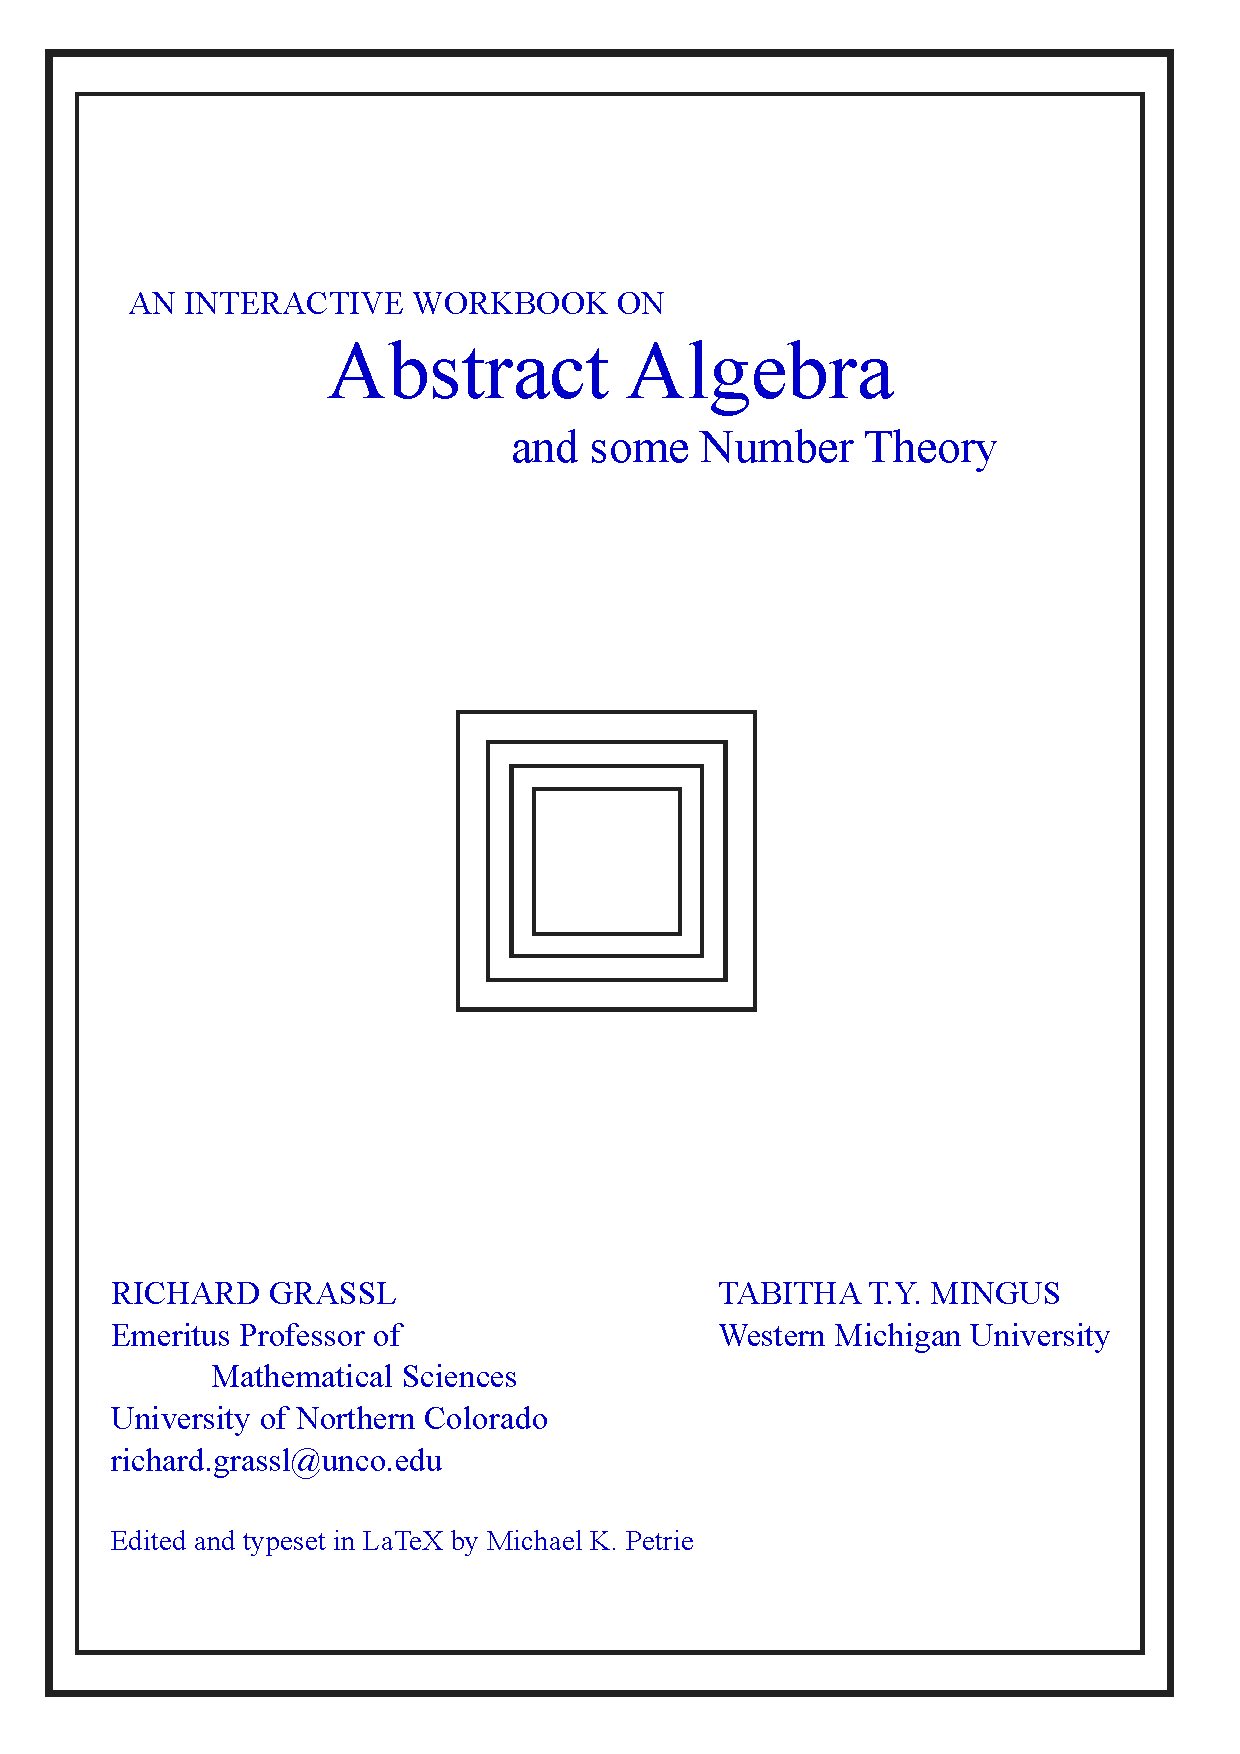
\includegraphics[width=6in]{coverpage2.pdf}}

\cleardoublepage

\includepdf[pages=2-]{workbook.pdf}

\cleardoublepage
\end{document}
